\RequirePackage{silence}
\documentclass[10pt,french,xcolor={svgnames,dvipsnames,x11names},trans]{beamer}

\usepackage{babel}
\usepackage{csquotes}
\usepackage{comment}
\usepackage{tikzsymbols}
\usepackage[utf8]{inputenc}

\usepackage{tcolorbox}
\usepackage{tabularx}
\usepackage{array}
\usepackage{colortbl}
\tcbuselibrary{skins}


%%% customisations
\usetheme[progressbar=frametitle]{metropolis}

%\usetheme[progressbar=frametitle,block=fill]{m}
\setmonofont[Scale=0.92]{Fira Mono}
\AtBeginSubsection{
\metroset{color/background=dark}
\frame[plain,c]{
  \begin{center}
  \begin{minipage}{25em}
    \usebeamercolor[fg]{section title}
    \usebeamerfont{section title}
    \insertsubsection\\[-1ex]
    \usebeamertemplate*{progress bar in section page}
  \end{minipage}
  \end{center}
}
\metroset{color/background=light}
}


\setbeamertemplate{frametitle continuation}[from second]
\usetikzlibrary{arrows}
\usetikzlibrary{chains}


\usepackage{tikz-qtree}
\usepackage{multicol}
\usepackage{relsize}
\usepackage{booktabs,tabularx}
\usepackage{listings}

\lstset{basicstyle=\ttfamily,breaklines=true,breakatwhitespace=true,
keywordstyle={\color{NavyBlue}\bfseries}, showstringspaces=false,
commentstyle={\color{PaleVioletRed4}},
emphstyle={\color{OliveGreen}\bfseries}
}

\newcolumntype{Y}{>{\raggedleft\arraybackslash}X}

\tcbset{tab1/.style={fonttitle=\bfseries\large,fontupper=\normalsize\sffamily,
colback=yellow!10!white,colframe=red!75!black,colbacktitle=Salmon!40!white,
coltitle=black,center title,freelance,frame code={
\foreach \n in {north east,north west,south east,south west}
{\path [fill=red!75!black] (interior.\n) circle (3mm); };},}}

\tcbset{tab2/.style={enhanced,fonttitle=\bfseries,fontupper=\normalsize\sffamily,
colback=yellow!0!white,colframe=OliveGreen!50!black,colbacktitle=Salmon!40!white,
coltitle=black,center title}}


\usepackage{algorithmic}
\renewcommand{\algorithmiccomment}[1]{\alert{/* #1 */}}


\makeatletter

\graphicspath{{figs/}}

\newcommand{\ccaption}[2]{\caption{\textbf{#1}#2}}
\newcommand{\sfig}[4]
{\begin{figure}[h]
    \centering
    \def\svgwidth{#2\textwidth}
    \input{./figs/#1.pdf_tex}
    \ccaption{#3}{#4}
    \label{fig_#1}
\end{figure}}

\renewcommand{\UrlFont}{\ttfamily}
\renewcommand{\vec}{\underline}

\title{Shared Memory Paradigm}

\subtitle{Methods for high performance computing}

\date{Février 2018\\SPHYM126\\[0.5ex]}
\author{Nicolas Roy}
\institute{
University of Namur
}

\begin{document}
\maketitle
\begin{frame}{Sommaire}
\setbeamertemplate{section in toc}[sections numbered]
\vspace*{\fill}
\tableofcontents[hideallsubsections]
\vspace*{\fill}
\end{frame}

\begin{frame}{Effective numeric performance}
    $$
    \mathcal{F} = \mathcal{C}_{\text{Cores}} * \mathcal{A}_{\text{AVX}} * \mathcal{V}_{\text{vector length}} * \mathcal{H}_{\text{Hyperthreading}} *\mathcal{F}_{\text{Freq}}
    $$
    Around 0.5 teraflops for a high-end laptop using stock overclock.
\end{frame}


\begin{frame}{Different parallel paradigms}
    \begin{figure}
        \centering
        \includegraphics[width=0.8\textwidth]{png/hyperthread.png}
    \end{figure}
\end{frame}


\begin{frame}{Hyperthreading - Corporate version}
    Shut-up, it's magic ! \emph{Intel}
    \begin{figure}
        \centering
        \includegraphics[width=0.8\textwidth]{png/intel_hyperthread.png}
    \end{figure}
\end{frame}

\begin{frame}{Hyperthreading - Honest version}
    Amazing (we cannot see the difference with real cores) for:
    \begin{itemize}
        \item Bad (for the meme) or heterogenous code
        \item Async, Async IO (Network operations, File access)
        \item Compiling your code
        \item Playing games (linked to first item)
        \item Battery, cost-per-unit
        \item Posting on messenger while your data gets Zucked
    \end{itemize}
    Ok (like sad 20\% improvement) for:
    \begin{itemize}
        \item Pure number crunching
    \end{itemize}
    Don't think there are downsides.
\end{frame}



\begin{frame}{Why should I care about SMP parallel programming ?}
    Embarrassingly parallel execution is king, unless
    \begin{itemize}
        \item Your task can be parallelized but is still heavily interlinked
        \item The algorithm is heavy and parallel (main sequence is long)
        \item You load a bunch of (common) data
        \item The main sequence is so small that process overhead is hard on you
    \end{itemize}
    \textbf{TL;DR:} You need \emph{Shared} memory.
\end{frame}
\begin{frame}{Different parallel paradigms}
    \begin{figure}
        \centering
        \includegraphics[width=1.0\textwidth]{pdf/parallelism.pdf}
    \end{figure}
\end{frame}
\begin{frame}{CPU architechture}
    \begin{figure}
        \centering
        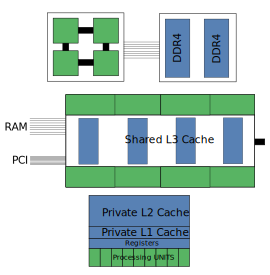
\includegraphics[width=1.0\textwidth]{pdf/architechture.pdf}
    \end{figure}
\end{frame}


\begin{frame}{Hyperthreading - Corporate version}
    Shut-up, it's magic ! \emph{Intel}
    \begin{figure}
        \centering
        \includegraphics[width=0.8\textwidth]{png/die.png}
    \end{figure}
\end{frame}
\plain{Code: Manipulations de base (C++)}





\plain{Merci de votre attention!}
\end{document}